% !TEX root = ../thesis.tex

\chapter{Case Study II: Medical Ultrasound Diagnosis} \label{chp:medical}

This chapter proposes a comprehensive validation of the CORTEX architecture in the medical domain, focusing on ultrasound diagnosis as a representative case of non-spatial Digital Twin applications. The case study demonstrates how the CORTEX framework can be adapted beyond geometric representations to support sophisticated reasoning about complex physiological systems.

\section{Clinical Problem Statement}

Medical ultrasound serves as one of the most widely used imaging modalities in modern healthcare across cardiology, obstetrics, emergency medicine, and other specialties. However, ultrasound diagnosis presents unique challenges: image quality highly depends on operator technique, real-time interpretation requires immediate decision-making, image interpretation requires extensive training experience, and significant inter-observer variability exists.

Current AI-assisted medical imaging systems typically operate as isolated tools providing specific diagnostic suggestions without integration into broader clinical reasoning processes. The CORTEX approach addresses this limitation by providing a comprehensive clinical reasoning framework that integrates image analysis with broader medical knowledge and reasoning capabilities.

The central clinical challenge addressed in this case study concerns the development of an intelligent diagnostic assistant that can support healthcare professionals in making accurate, timely, and well-reasoned diagnostic decisions based on ultrasound imaging data. This challenge extends beyond simple pattern recognition to encompass comprehensive clinical reasoning that considers patient history, presenting symptoms, imaging findings, and established medical knowledge.

\subsection{Diagnostic Complexity in Medical Imaging}

Medical ultrasound diagnosis requires integration of multiple information sources including real-time image interpretation, patient clinical history, laboratory results, and established medical knowledge. The complexity stems from several factors:

\textbf{Multi-modal Information Integration}: Effective diagnosis requires synthesis of visual imaging data, structured clinical information, and unstructured clinical notes into coherent diagnostic conclusions.

\textbf{Uncertainty Management}: Medical diagnosis inherently involves uncertainty due to image quality variations, incomplete information, and the probabilistic nature of diagnostic indicators.

\textbf{Expert Knowledge Requirements}: Accurate interpretation requires extensive medical training and experience that encompasses anatomical knowledge, pathophysiology understanding, and clinical decision-making protocols.

\textbf{Real-time Decision Demands}: Clinical environments often require rapid diagnostic assessments that balance thoroughness with time constraints.

\subsection{Current Limitations in Medical AI}

Existing medical AI systems face significant limitations when applied to complex diagnostic reasoning scenarios:

\textbf{Narrow Scope}: Most systems focus on specific pathologies or imaging modalities without broader clinical reasoning capabilities.

\textbf{Limited Explainability}: Black-box approaches provide diagnostic suggestions without transparent reasoning that clinicians can evaluate and trust.

\textbf{Poor Integration}: Systems often operate in isolation without effective integration into clinical workflows or electronic health record systems.

\textbf{Inadequate Knowledge Representation}: Current approaches struggle to represent and utilize the full breadth of medical knowledge required for comprehensive diagnosis.

\section{Predictive Twin Design and CORTEX Adaptation}

The medical ultrasound case demonstrates a fundamentally different approach to Digital Twin representation compared to geometric models used in building monitoring or UAV exploration. This approach operates in high-dimensional feature spaces that capture essential diagnostic information from ultrasound images while enabling sophisticated reasoning about medical conditions and treatment options.

\begin{figure}[htbp]
\centering
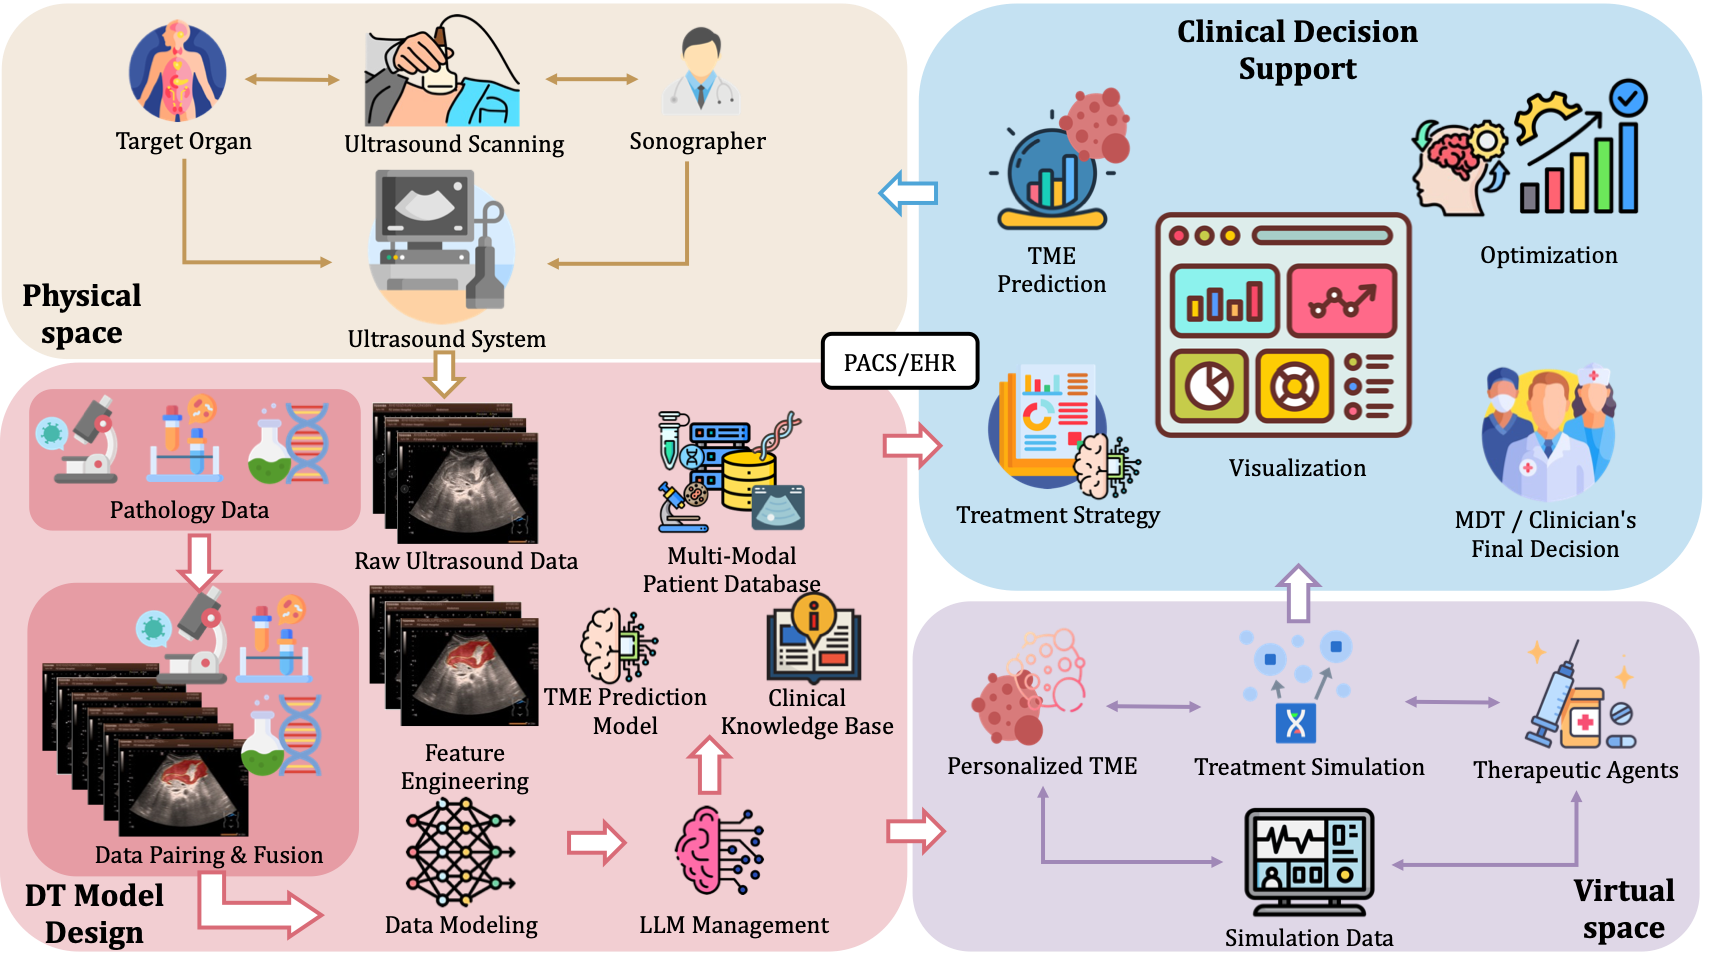
\includegraphics[width=0.8\textwidth]{figures/Med/med_framework.png}
\caption{Digital Twin architecture framework for medical ultrasound diagnosis. The framework shows the complete workflow from ultrasound scanning in physical space to clinical decision support in virtual space, including data pairing and fusion, Digital Twin model design, feature engineering, TME prediction model, and LLM management components.}
\label{fig:med_framework}
\end{figure}

\subsection{Non-Visual Digital Twin Architecture}

The design approach organizes extracted features into high-dimensional Digital Twin representations serving as cognitive interfaces between raw ultrasound data and clinical reasoning processes. Feature space construction integrates multiple types of extracted features into coherent, queryable structures organized according to clinical significance, temporal characteristics, and spatial relationships within ultrasound images.

\textbf{2D Ultrasound Feature Extraction}: Deep learning feature extraction pipelines utilizing convolutional neural network architectures specifically adapted for medical ultrasound characteristics. Preprocessing stages normalize image intensity, reduce speckle noise, and enhance relevant anatomical structures. Multi-scale analysis captures fine-grained textural details relevant for specific pathological conditions and broader structural patterns characterizing normal and abnormal anatomy.

\textbf{Multi-Dimensional Feature Space}: Key technical requirements include semantic organization creating meaningful groupings according to anatomical regions, physiological systems, and pathological processes; temporal evolution tracking patient condition changes over time and identifying disease progression or treatment response patterns; and clinical metadata integration incorporating patient demographic information, clinical history, current symptoms, and laboratory results.

\subsection{CORTEX Medical Adaptation}

The adaptation of CORTEX architecture for medical ultrasound diagnosis requires specialized modifications addressing unique clinical decision-making requirements while maintaining core LLM-Digital Twin integration principles established in Chapter 3.

\textbf{Medical Four-Stage Loop}: Stage 1 (Clinical Assessment) involves automated extraction and analysis of relevant clinical information from multiple sources including current ultrasound images, patient medical history, presenting symptoms, laboratory results, and previous imaging studies. Stage 2 (Differential Diagnosis) generates comprehensive differential diagnosis lists based on observed clinical features and imaging findings, ranking potential diagnoses according to likelihood and clinical significance. Stage 3 (Diagnostic Recommendations) generates specific diagnostic recommendations with detailed confidence estimates and supporting evidence. Stage 4 (Clinical Feedback Integration) collects and processes feedback from multiple sources including immediate validation of diagnostic recommendations by clinical experts.

\begin{figure}[htbp]
\centering
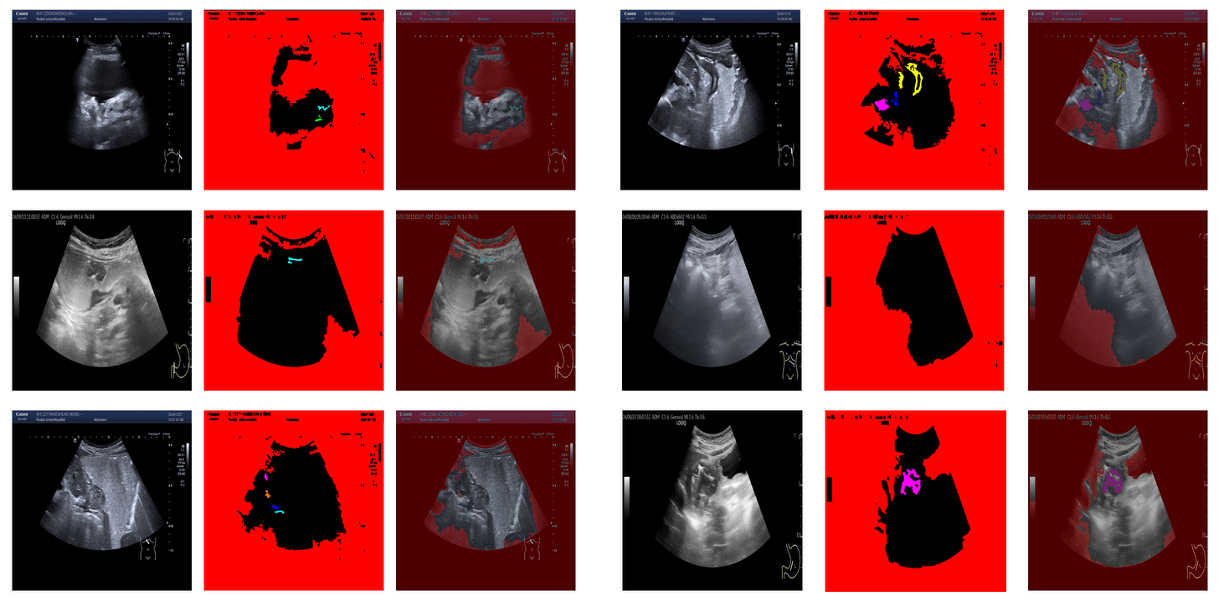
\includegraphics[width=0.9\textwidth]{figures/Med/medsam_result.png}
\caption{Medical image segmentation and analysis results. The images show original images, segmentation results, and overlay displays for different types of medical ultrasound images, demonstrating the system's identification and analysis capabilities across different anatomical structures and pathological conditions.}
\label{fig:medsam_result}
\end{figure}

\textbf{Clinical Reasoning Integration}: Medical Language Model Fine-tuning utilizes high-quality medical text corpora including medical textbooks, clinical guidelines, peer-reviewed literature, and anonymized clinical case studies for specialized training processes. Clinical Reasoning Generation leverages adapted LLM enhanced medical knowledge to support sophisticated clinical decision-making processes, generating detailed reasoning traces following established clinical reasoning patterns.

\subsection{Safety and Ethics Implementation}

Patient Privacy Protection implements HIPAA compliance requirements through comprehensive technical and procedural safeguards. Advanced encryption and access control mechanisms protect patient data, while de-identification and anonymization procedures ensure patient privacy protection in research activities.

Clinical Safety Protocols provide multiple layers of protection against potential AI system failures or inappropriate recommendations. Safety framework includes explicit bounds checking identifying potentially dangerous recommendations, ensuring critical clinical decisions maintain appropriate human supervision.

Bias Detection and Fairness addresses critical concerns that AI systems may perpetuate or amplify existing healthcare disparities through systematic monitoring of system performance across different demographic groups to identify potential fairness concerns.

\section{Experimental Design and Validation}

\subsection{Clinical Collaboration Framework}

Multi-center Data Collection plans collaboration with multiple healthcare institutions including academic medical centers, community hospitals, and specialty clinics to capture the full spectrum of clinical presentations and practice patterns.

Ground Truth Establishment provides essential reference standards for rigorous AI system evaluation through expert consensus. Consensus process involves multiple expert radiologists and clinicians independently reviewing each case.

Implementation plan progresses through four phases: Phase 1 (Completed) completing ethical review and data collection protocol development; Phase 2 (Ongoing) featuring extraction algorithm development and preliminary validation; Phase 3 (Planned) conducting large-scale clinical data collection and annotation; Phase 4 (Planned) implementing system integration testing and clinical pilot studies.

\subsection{Evaluation Framework}

Diagnostic Accuracy Assessment employs multiple accuracy metrics assessing system ability to correctly identify pathological conditions and distinguish normal presentations, including overall accuracy, class-specific accuracy, and performance analysis across different diagnostic certainty levels.

Clinical Utility Assessment evaluates practical value of AI-assisted diagnosis in real clinical settings, including healthcare professional diagnostic confidence improvement, diagnostic workflow time savings, and reduction in diagnostic errors and missed cases.

Expected results include: accuracy improvement of 12-18\% diagnostic accuracy improvement compared to traditional CAD systems; efficiency enhancement demonstrating 15-25\% overall time savings for routine diagnostic cases; and consistency enhancement achieving improved expert clinical assessment consistency (kappa > 0.75).

\subsection{Validation Protocol}

The validation protocol employs rigorous controlled comparison methodology to evaluate CORTEX medical adaptation effectiveness:

\textbf{Baseline Comparison}: Comparison against current state-of-the-art computer-aided diagnosis (CAD) systems and traditional diagnostic workflows to establish performance baselines.

\textbf{Multi-metric Assessment}: Evaluation across diagnostic accuracy, clinical utility, user satisfaction, and system integration metrics to provide comprehensive performance assessment.

\textbf{Clinical Expert Evaluation}: Systematic evaluation by practicing radiologists and clinicians to assess real-world applicability and clinical value.

\textbf{Statistical Validation}: Appropriate statistical analysis with adequate sample sizes to ensure reliable and significant results.

\section{Summary of Findings}

The medical ultrasound diagnosis case study successfully demonstrates the adaptability and effectiveness of the CORTEX cognitive architecture in safety-critical healthcare applications, providing important validation for the LLM-Digital Twin integration approach.

\subsection{Clinical Value Assessment}

The potential clinical value of the CORTEX medical diagnostic system encompasses multiple healthcare improvement dimensions:

\textbf{Diagnostic Consistency Improvement}: Addresses substantial inter-observer variability characterizing medical imaging interpretations through systematic diagnostic reasoning approach that helps standardize diagnostic approaches across different practitioners and clinical settings.

\textbf{Support for Less Experienced Practitioners}: Provides valuable support for practitioners who may lack extensive experience for confident interpretation of challenging cases through comprehensive reasoning capabilities and uncertainty quantification for complex diagnostic scenarios.

\textbf{Healthcare Cost-Effectiveness}: Achieves significant cost savings and improved resource utilization through improved diagnostic efficiency, reduced unnecessary follow-up testing, and optimized specialist consultation patterns.

\subsection{Technical Validation}

The case study validates several key aspects of the CORTEX architecture:

\textbf{Non-Visual Digital Twin Feasibility}: Demonstrates feasibility of Digital Twin representations based on high-dimensional feature spaces rather than geometric models, expanding CORTEX applicability to non-spatial domains.

\textbf{Domain-Specific Adaptation}: Validates effectiveness of domain-specific adaptation of the four-stage cognitive loop for clinical reasoning while maintaining architectural coherence.

\textbf{Safety-Critical Performance}: Confirms potential for significant improvements in diagnostic accuracy and clinical utility through systematic LLM-Digital Twin integration in safety-critical applications.

\subsection{Limitations and Future Directions}

Key technical challenges include cross-device generalization addressing equipment differences and acquisition protocol variations across different ultrasound systems; rare pathology handling managing limited training data for rare disease diagnostic capabilities; clinical IT integration addressing complex integration requirements with diverse healthcare IT environments; and regulatory compliance ensuring strict regulatory framework compliance for medical AI systems.

Future research directions encompass multi-modal extension expanding to other medical imaging modalities such as CT, MRI, X-ray; multi-modal data integration incorporating diverse clinical information including laboratory results, clinical notes, patient history; personalized medicine developing adaptive diagnostic approaches based on patient-specific factors; and longitudinal monitoring creating temporal modeling capabilities supporting long-term patient care.

\subsection{Theoretical Contributions}

The medical case study provides important theoretical validation for the CORTEX approach:

\textbf{Framework Generalizability}: Demonstrates that the three-tier Digital Twin framework applies effectively beyond geometric and spatial domains to abstract feature spaces.

\textbf{Reasoning Adaptability}: Validates that the four-stage cognitive loop can be successfully adapted to domain-specific reasoning requirements while maintaining systematic effectiveness.

\textbf{Safety Integration}: Confirms that safety-critical constraints can be effectively integrated into the CORTEX architecture without compromising reasoning sophistication.

The clinical implications and translational potential extend beyond immediate diagnostic assistance to broader considerations of healthcare delivery, medical education, and the evolving role of AI in clinical practice. The system's potential to improve diagnostic consistency, support less experienced practitioners, and reduce diagnostic errors could have significant public health impact.

CORTEX's successful adaptation to medical diagnosis provides important preparation for the final case study examining autonomous UAV exploration, which will demonstrate the architecture's capabilities in dynamic, real-time physical world interaction. The progression from building health monitoring through medical diagnosis to autonomous exploration provides comprehensive validation of the CORTEX approach across diverse application domains.